\chapter{Pruebas}\label{chapter:testing}

A continuación se describen las pruebas realizadas para validar el sistema implementado, las pruebas se dividieron en 2 tipos: backend y frontend. Para las del backend se crearon tests automáticos probando varios de los endpoints de la aplicación, en el caso del frontend se hicieron varios experimentos interactuando directamente con la interfaz web.

\section{Backend}

Para comprobar que todo funcionaba correctamente se prepararon varias pruebas, se crearon 500 usuarios: 100 con nombres \textit{'estudiante1'}, \textit{'estudiante2}, ... , \textit{estudiante100}, otros 100 con nombre \textit{'clasificador1'}, ... \textit{clasificador100}, y así con el resto de los roles, luego de esto se verificó que existían 501 usuarios, un administrador que se crea automáticamente al ejecutar el backend por primera vez, y los 500 creados en la prueba, se verificó que existían 100 de cada grupo leyendo los prefijos en sus nombres.
\newline

Luego, usando el administrador creado por defecto, se le cambió el rol a cada usuario dependiendo de su nombre, a los que tenían prefijo 'estudiante' se le asignó dicho rol, igualmente con el resto de los roles. Al concluir se verificó que los prefijos en los nombres coincidían con el rol de cada usuario.
\newline

También se crearon satisfactoriamente 5 áreas, llamadas \textit{'area1'}, \textit{'area2'}, ... y \textit{'area5'}, y se le asignó a cada especialista con \textit{'id mod 5 = i'} el \textit{'areai'}, la operación fue realizada con éxito.
\newline

Luego, con cada estudiante se escribió una pregunta, y con un clasificador se clasificó cada pregunta siguiendo el mismo patrón de las áreas de los especialistas. Con un especialista de cada área se tomaron las preguntas satisfactoriamente, las que provenían de estudiantes con id par se respondieron, y las de otras se subieron de nivel; con estas últimas se aplicó un procedimiento similar respondiendo las de estudiantes con id divisible por 4 y subiendo a la administración el resto para finalmente darles respuestas. Se comprobó durante todo el proceso que las tareas iban según lo planeado.
\newline

\section{Frontend}

En este caso se prepararon varias tareas (se muestran algunas capturas de pantalla):
\begin{itemize}
	\item Registrarse con un usuario llamado f\_estudiante: se debe entrar a la página, presionar en el botón \textit{'Registrarse'} y rellenar los datos (al desmarcar la opción de \textit{'Soy trabajador de MATCOM'} el usuario es creado en el rol de estudiante) (figura \ref{fig:f_estudiante_registro}).
	
	\item Registrarse con un usuario llamado f\_clasificador: se debe cerrar sesión y aplicar el mismo procedimiento del punto anterior (al marcar la opción \textit{'Soy trabajador de MATCOM'} el usuario es creado con el rol de clasificador).
	
	\item Registrarse con otros 2 usuarios, uno llamado f\_especialista1 y otro f\_especialista2.
	
	\item Iniciar sesión con el administrador y asignarle el rol \textit{'Especialista Nivel 1'} al usuario con nombre f\_especialista1, y \textit{'Especialista Nivel 2'} a f\_especialista2: para esto se debe cerrar sesión, iniciar sesión con el administrador (correo: admin@admin.com, contraseña: administrador), ir a la sección de usuarios, buscar al usuario en cuestión y cambiarle el rol (figura \ref{fig:f_cambio_rol}).
	
	\item  Crear un área con el nombre \textit{'f\_area'}: esto se hace en la sección de áreas (figura \ref{fig:f_crear_ara}).
	
	\item Asignarle el área \textit{f\_area} a los usuarios f\_especialista1 y f\_especialista2, esto se lleva a cabo en la sección de usuarios (figura \ref{fig:f_cambiar_area}).
	
	\item Iniciar sesión con f\_estudiante y escribir 3 preguntas (figura \ref{fig:f_crear_pregunta}). Luego entrar a la sección \textit{'Mis dudas'} y verificar que estén creadas las preguntas (figura \ref{fig:f_verificar_crear_preguntas}).
	
	\item Iniciar sesión con f\_clasificador y clasificar las 3 preguntas creadas en el punto anterior en el área \textit{'f\_area'} (figura \ref{fig:f_clasificar_preguntas}).
	
	\item Iniciar sesión con f\_especialista1 y tomar las 3 preguntas, esto se hace desde la sección \textit{'Preguntas clasificadas'} (figura \ref{fig:f_tomar_preguntas1}). Luego se debe ir a la sección \textit{'Mis preguntas'} y verificar que las dudas estén ahí (figura \ref{fig:f_virificar_preguntas_tomadas1}).
	
	\item Responder la pregunta \textit{'pregunta 1'} y subir de nivel las otras 2 (figura \ref{fig:f_subir_nivel_2}). Luego iniciar sesión con f\_estudiante y verificar que tiene respuesta en la pregunta 1 (figura \ref{fig:f_verificar_respuesta1}), también se debe ingresar con f\_especialista2 y ver si le aparecen las preguntas \textit{'pregunta 2'} y \textit{'pregunta 3'} (figura \ref{fig:f_verificar_subida2}).
	
	\item Iniciar sesión con f\_especialista2 y tomar las 2 preguntas (pregunta 1 y pregunta 2), responder la 2 y subir de nivel la 3 (figura \ref{fig:f_subida3}). Verificar con f\_estudiante que la pregunta 2 tiene respuesta (figura \ref{fig:f_respuesta2}) y con el administrador que le aparece la pregunta 3 (figura \ref{fig:f_verificacion_admin}).
	
	\item Con el administrador tomar la pregunta 3, chatear con el estudiante (figura \ref{fig:f_chat_admin}) y finalmente darle respuesta (figura \ref{fig:f_respuesta3}).
\newline

	
Todos los tests pasaron satisfactoriamente por lo que el sistema está listo para ser lanzado.
	
\end{itemize}


	\begin{figure}[h]
		\begin{center}
		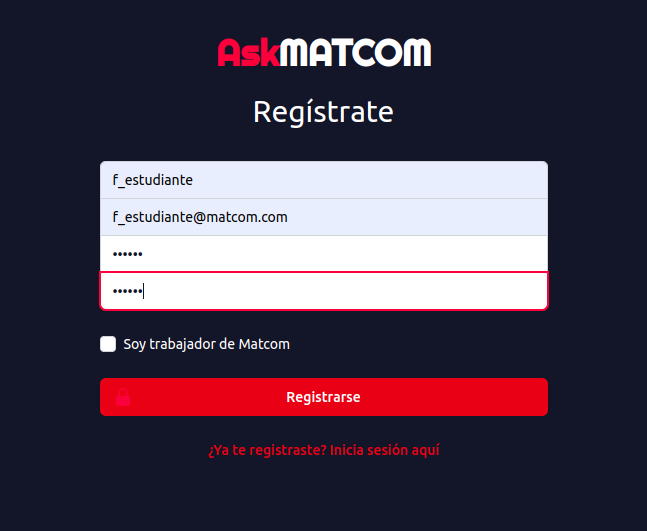
\includegraphics[width=6cm, height=5cm]{registro_f_estudiante.png}
		\caption{Registro de f\_estudiante}
		\label{fig:f_estudiante_registro}
		
	\end{center}
	\end{figure}

	\begin{figure}[h]
	\begin{center}
		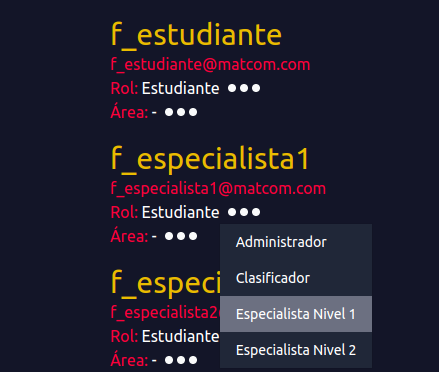
\includegraphics[width=6cm, height=5cm]{cambio_rol.png}
		\caption{Cambio de rol}
		\label{fig:f_cambio_rol}
		
	\end{center}
\end{figure}

	\begin{figure}[h]
	\begin{center}
		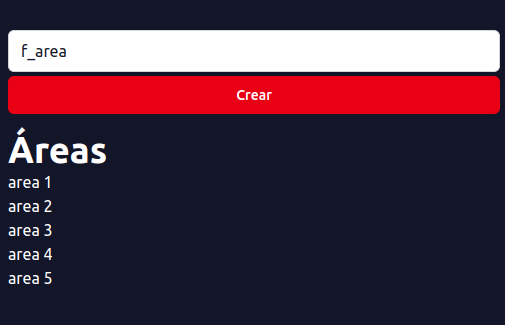
\includegraphics[width=6cm, height=5cm]{crear_area.png}
		\caption{Crear área}
		\label{fig:f_crear_ara}
		
	\end{center}
\end{figure}

	\begin{figure}[h]
	\begin{center}
		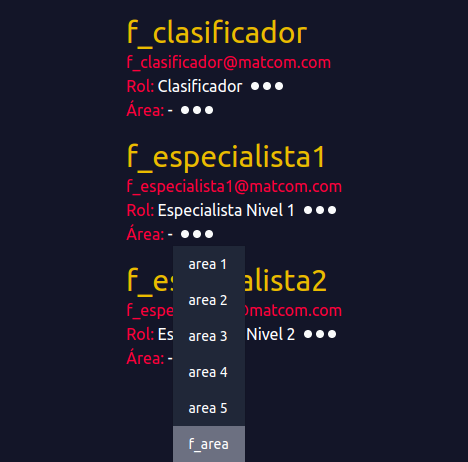
\includegraphics[width=6cm, height=5cm]{cambiar_area.png}
		\caption{Cambiar área}
		\label{fig:f_cambiar_area}
		
	\end{center}
\end{figure}

\begin{figure}[h]
	\begin{center}
		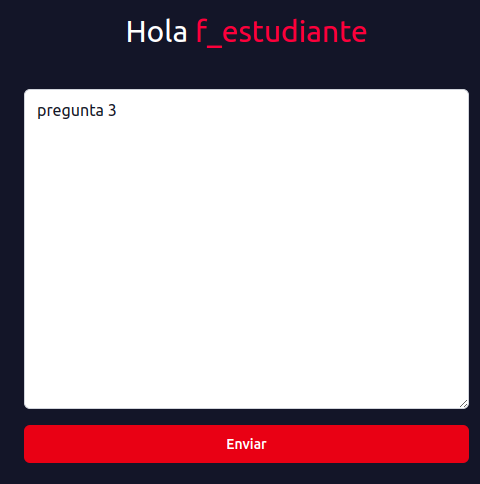
\includegraphics[width=6cm, height=5cm]{crear_pregunta.png}
		\caption{Crear preguntas}
		\label{fig:f_crear_pregunta}
		
	\end{center}
\end{figure}

\begin{figure}[h]
	\begin{center}
		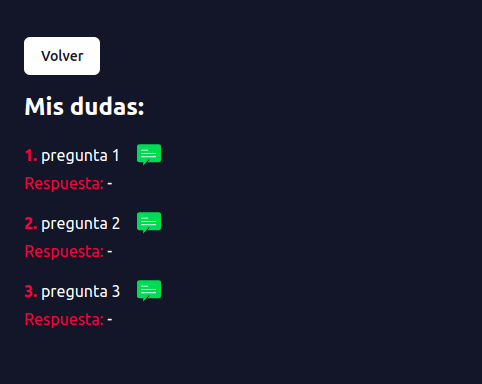
\includegraphics[width=6cm, height=5cm]{verificar_crear_preguntas.png}
		\caption{Verificación de la creación de las preguntas}
		\label{fig:f_verificar_crear_preguntas}
		
	\end{center}
\end{figure}

\begin{figure}[h]
	\begin{center}
		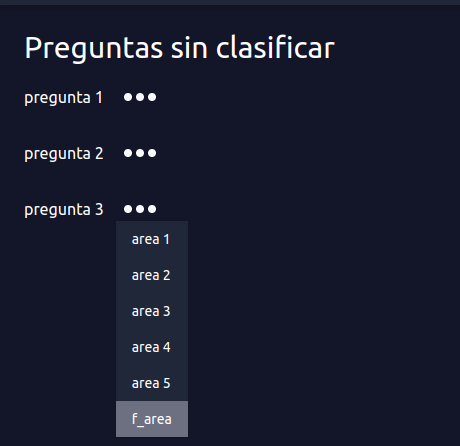
\includegraphics[width=6cm, height=5cm]{clasificar_preguntas.png}
		\caption{Clasificar preguntas}
		\label{fig:f_clasificar_preguntas}
		
	\end{center}
\end{figure}

\begin{figure}[h]
	\begin{center}
		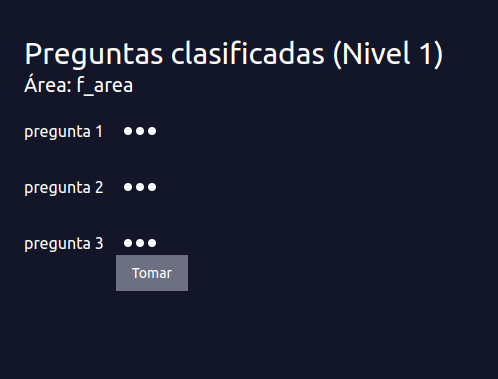
\includegraphics[width=6cm, height=5cm]{tomar_preguntas.png}
		\caption{Tomar preguntas con el especialista de nivel 1}
		\label{fig:f_tomar_preguntas1}
		
	\end{center}
\end{figure}

\begin{figure}[h]
	\begin{center}
		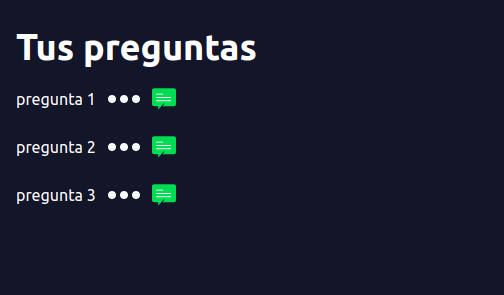
\includegraphics[width=6cm, height=5cm]{verificar_preguntas_tomadas.png}
		\caption{Verificación de que las preguntas fueron tomadas}
		\label{fig:f_virificar_preguntas_tomadas1}
		
	\end{center}
\end{figure}

\begin{figure}[h]
	\begin{center}
		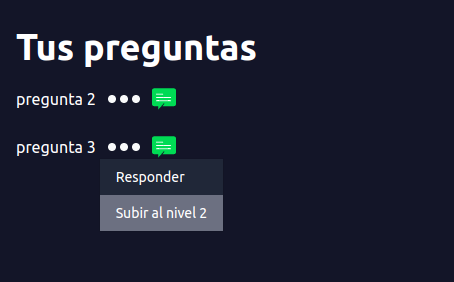
\includegraphics[width=6cm, height=5cm]{subir_nivel_2.png}
		\caption{Subida de nivel de las preguntas 2 y 3}
		\label{fig:f_subir_nivel_2}
		
	\end{center}
\end{figure}

\begin{figure}[h]
	\begin{center}
		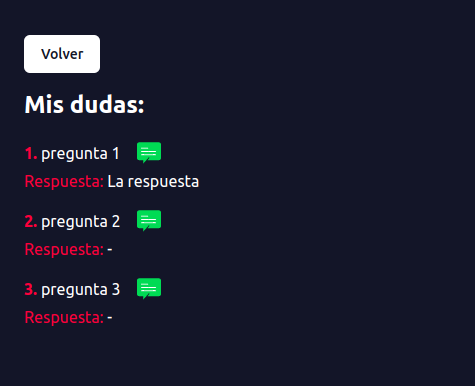
\includegraphics[width=6cm, height=5cm]{verificar_respuesta_1.png}
		\caption{Verificación de la respuesta a la pregunta 1}
		\label{fig:f_verificar_respuesta1}
		
	\end{center}
\end{figure}

\begin{figure}[h]
	\begin{center}
		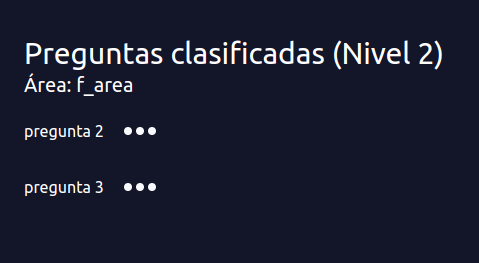
\includegraphics[width=6cm, height=5cm]{verificar_subida_2.png}
		\caption{Verificación de la subida de nivel de las preguntas 2 y 3}
		\label{fig:f_verificar_subida2}
		
	\end{center}
\end{figure}

\begin{figure}[h]
	\begin{center}
		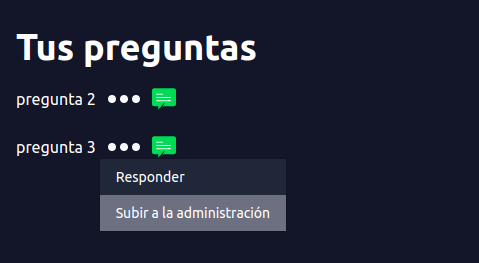
\includegraphics[width=6cm, height=5cm]{subida_nivel3.png}
		\caption{Subida a la administración de las preguntas 2 y 3}
		\label{fig:f_subida3}
		
	\end{center}
\end{figure}

\begin{figure}[h]
	\begin{center}
		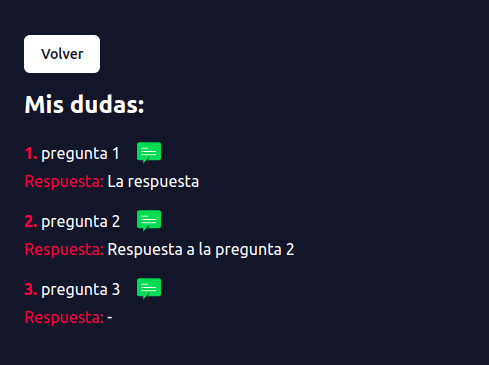
\includegraphics[width=6cm, height=5cm]{respuesta2.png}
		\caption{Verificación de la respuesta a la pregunta 2}
		\label{fig:f_respuesta2}
		
	\end{center}
\end{figure}

\begin{figure}[h]
	\begin{center}
		
\includegraphics[width=6cm, height=5cm]{verificar_subida3.png}
		\caption{Verificación de la subida a la administración de la pregunta 3}
		\label{fig:f_verificacion_admin}
		
	\end{center}
\end{figure}


\begin{figure}[h]
	\begin{center}
		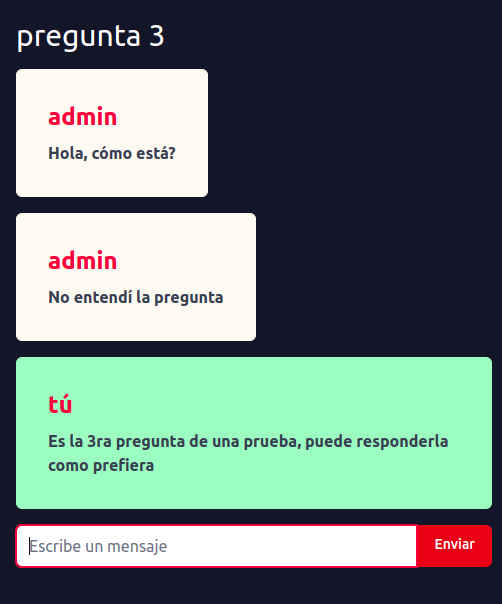
\includegraphics[width=6cm, height=5cm]{chat_admin.png}
		\caption{Chat entre el administrador y f\_estudiante}
		\label{fig:f_chat_admin}
		
	\end{center}
\end{figure}

\begin{figure}[h]
	\begin{center}
		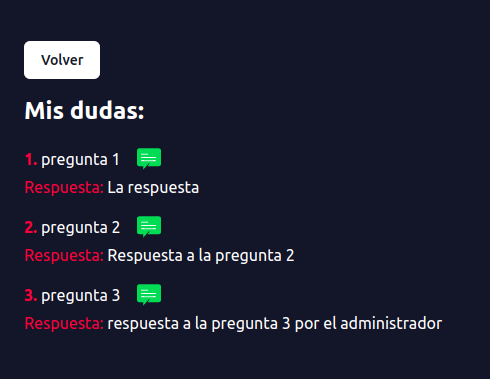
\includegraphics[width=6cm, height=5cm]{respuesta3.png}
		\caption{Verificación de la respuesta a la pregunta 3}
		\label{fig:f_respuesta3}
		
	\end{center}
\end{figure}
